\documentclass[12pt]{article}
\usepackage{graphicx}
\usepackage{subfigure}
\usepackage{epsfig}
\pagestyle{empty}

\begin{document}

\title{Problem B \\ Magetic Stones}
\author{Input file: {\em PB.in} \\ Time limit: 2 seconds}
\date{}
\maketitle
\thispagestyle{empty}

\subsection*{Problem Description}
Astronauts discovered a new planet in rich of a variety of magnetic stones never seen on earth.
These magnetic stones can be distinguished by 26 colors. Each magnetic stone can only have either one of two opposite poles, similar to the north pole (N) and south pole (S) on earth. Only magnetic stones having the same colors and carrying opposite poles can be attracted.
These stones release tremendous energy when two opposite poles of magnets are attracted together. 
Therefore, human beings decide to massively dig out these stones from rocks for collection of energy.
However, these magnetic stones are initially linearly-arranged in a chain in the rocks by an unknown mysterious force. When a chain of stones are pulled out from the rock and thrown to the floor, a pair of stones with the same color and opposite poles can be attracted. And the entire chain of stones will be eventually self-folded into a hairpin-like structure, and trememdous energy will be released during this process.
Scientists observed that the released energy is proportional to the number of attracted magnetic stones and reduced by the remaining stones, including repelled stones and singleton/hanging stones. Each pair of attracted stones will generate 2 joules of energy, whereas each pair of repelled stones, as well as each singleton/hanging stones, will reduce 1 joule. For example (Fig. (a)), the chain of stones will be self-folded and release 3 joules at the end, as three pairs of stones with opposite poles are attracted and generate 6 joules, while two pairs of repelled stones and one singleton stone (on the loop) reduce 3 joules. Note that the stones can be self-folded into multiple planar hairpin structures in order to maximize the released energy (Fig. (b)). Given a linear chain of stones, you are asked to compute the maximum energy these stones will release.


 \begin{figure}[!h]
        \centering
        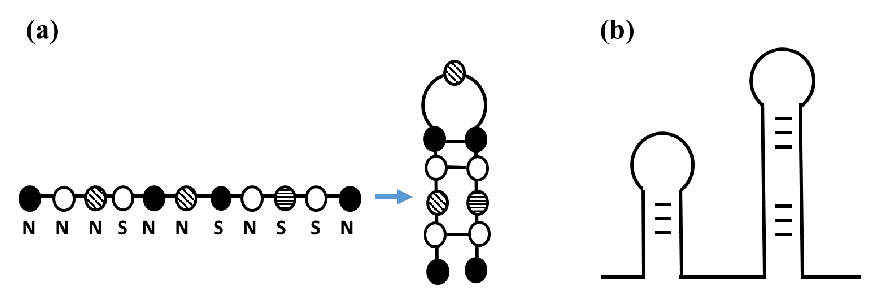
\includegraphics[scale=0.8]{Fig.eps}
        \end{figure}
        
\subsection*{Input Format}

The first line contains a positive integer standing for the number of test cases. Each following line is one test case. Each test case contains a chain of stones represented by a string. The 26 colors are represented using the standard alphabet (from a to z and from A to Z). The two opposite poles of stones with the same color are represented as upper and lower cases (e.g., a and A stands for two stones with the same color and opposite poles).

\subsection*{Output Format}

Each line of the output corresponds to the output of each test case. Each line will consist of an integer, which is the maximum joules released by the chain of stones.

\subsection*{Sample Input}
\begin{verbatim}
3
ABCbACaBdbA
GHTUIOoiuthg
AGCBhhbcg
\end{verbatim}

\subsection*{Sample Output}
\begin{verbatim}
3
12
4
\end{verbatim}
\end{document}
